\documentclass[pdflatex,compress]{beamer}

%\usetheme[dark,framenumber,totalframenumber]{ElektroITK}
\usetheme[darktitle,framenumber,totalframenumber]{ElektroITK}
\usepackage[utf8]{inputenc}
\usepackage[T1]{fontenc}
\usepackage{lmodern}
%\usepackage[bahasai]{babel}
\usepackage{amsmath}
\usepackage{amsfonts}
\usepackage{amssymb}
\usepackage{graphicx}
\usepackage{multicol}
\usepackage{lipsum}
\usefonttheme[onlymath]{serif}

\newcommand*{\Scale}[2][4]{\scalebox{#1}{$#2$}}%

\setbeamertemplate{caption}[numbered]

\AtBeginSection[]{
	\begin{frame}
		\vfill
		\centering
		\usebeamerfont{title}\insertsectionhead\par%
		\vfill
	\end{frame}
}

\title{Electronic Circuit II}
\subtitle{Comparator}

\author{Mifta Nur Farid}

\begin{document}

\maketitle

\section{Comparators with Zero Reference}

\begin{frame}
	\frametitle{Introduction}
	\begin{itemize}
		\item Often we want to compare one voltage with another to see which is larger.
		\item In this situation, a comparator may be the perfect solution.
		\item A comparator is similar to an op amp because it has two input voltages (noninverting and inverting) and one output voltage.
		\item It differs from a linear op-amp circuit because it has a two-state output, either a low or a high voltage.
		\item Because of this, comparators are often used to interface with analog and digital circuits.
	\end{itemize}
\end{frame}

\begin{frame}
	\frametitle{Basic Idea}
	\begin{multicols}{2}
		\begin{itemize}
			\item The simplest way to build a comparator is to connect an op amp without feedback resistors, as shown in Fig. \ref{fig:img01}.
		\end{itemize}
		\columnbreak
		\begin{figure}
			\centering
			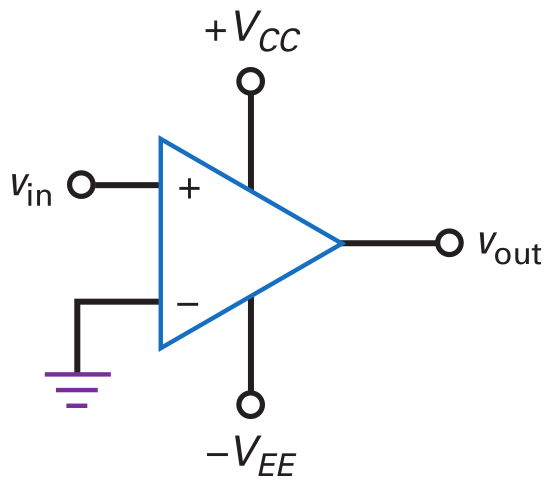
\includegraphics[width=0.7\linewidth]{img/img01}
			\caption{Comparator}
			\label{fig:img01}
		\end{figure}
	\end{multicols}
\end{frame}

\begin{frame}{Basic Idea}
	\begin{itemize}
		\item Because of the high open-loop voltage gain, a positive input voltage produces positive saturation, and a negative input voltage produces negative saturation.
		\item The comparator of Fig. \ref{fig:img01} is called \textbf{a zero-crossing detector} because the output voltage ideally switches from low to high or vice versa whenever the input voltage crosses zero.
	\end{itemize}
\end{frame}

\begin{frame}{Basic Idea}
	\begin{multicols}{2}
		\begin{itemize}
			\item Figure \ref{fig:img02} shows the input-output response of a
			zero-crossing detector.
		\end{itemize}
		\columnbreak
		\begin{figure}
			\centering
			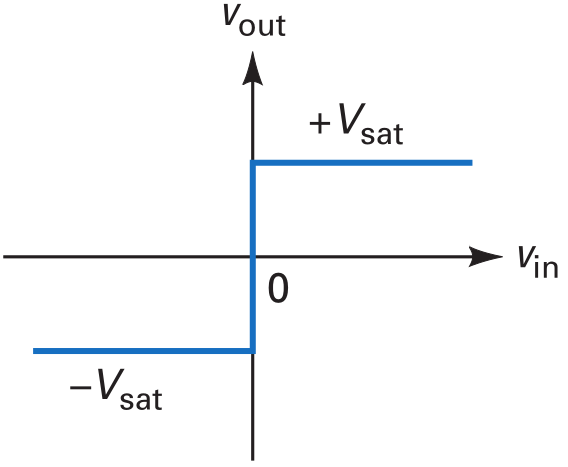
\includegraphics[width=0.7\linewidth]{img/img02}
			\caption{Input/output response}
			\label{fig:img02}
		\end{figure}
	\end{multicols}
\end{frame}

\begin{frame}{Basic Idea}
	\begin{itemize}
		\item The minimum input voltage that produces saturation is:
		\begin{equation}\label{eq:01}
			v_{in(min)} = \frac{\pm V_{sat}}{A_{VOL}}
		\end{equation}
		\item If $V_{sat}$ = 14 V, the output swing of the comparator is from approximately -14 to +14 V.
		\item If the open-loop voltage gain is 100,000, the input voltage needed to produce saturation is:
		\begin{equation*}
			v_{in(min)} = \frac{\pm V_{sat}}{A_{VOL}} = \frac{\pm 14 \text{ V}}{100,000} = \pm 0.14 \text{ mV}
		\end{equation*}
	\end{itemize}
\end{frame}

\begin{frame}{Basic Idea}
	\begin{itemize}
		\item This means that an input voltage more positive than +0.140 mV drives the comparator into positive saturation, and an input voltage more negative than -0.140 mV drives it into negative saturation.
		\item Input voltages used with comparators are usually much greater than
		$\pm$0.140 mV.
		\item This is why the output voltage is a two-state output, either $+V_{\text{sat}}$ or $-V_{\text{sat}}$.
		\item By looking at the output voltage, we can instantly tell whether the input voltage is greater than or less than zero.
	\end{itemize}
\end{frame}

\begin{frame}
	\frametitle{Lissajous Pattern}
	\begin{itemize}
		\item A \textbf{Lissajous pattern} appears on an oscilloscope when harmonically related signals are applied to the horizontal and vertical inputs.
		\item One convenient way to display the input/output response of any circuit is with a Lissajous pattern in which the two harmonically related signals are the input and output voltages of the circuit.
	\end{itemize}
\end{frame}

\begin{frame}{Lissajous Pattern}
	\begin{itemize}
		\item For instance, Fig. \ref{fig:img03} shows the input/output response for a 741C with supplies of $\pm$15 V.
	\end{itemize}
	\begin{figure}
		\centering
		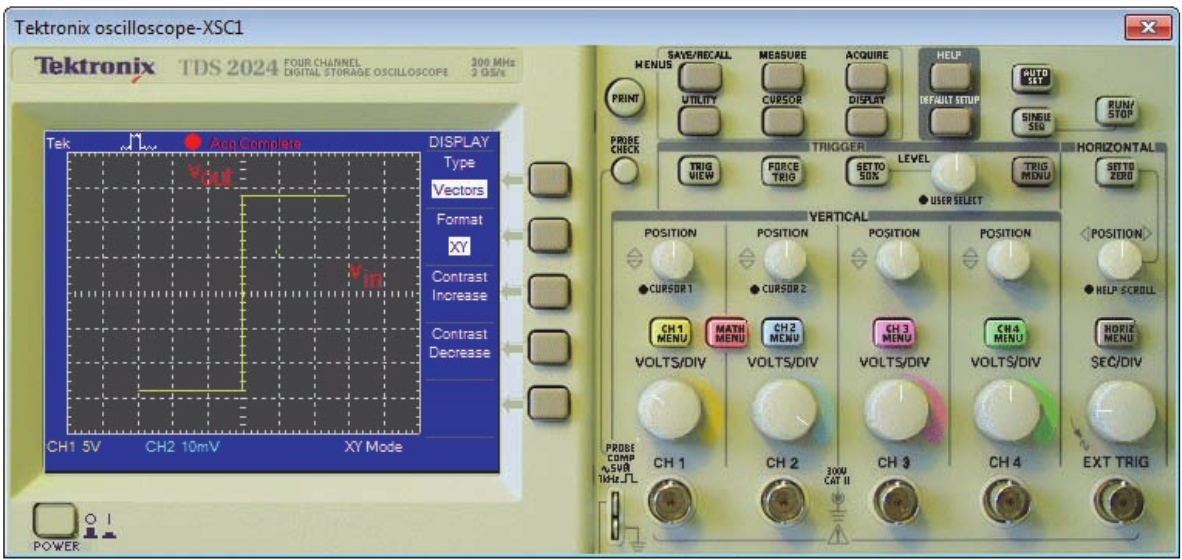
\includegraphics[width=\linewidth]{img/img03}
		\caption{741C response}
		\label{fig:img03}
	\end{figure}
\end{frame}

\begin{frame}{Lissajous Pattern}
	\begin{itemize}
		\item Channel 1 (the vertical axis) has a sensitivity of 5 V/Div. As
		we can see, the output voltage is either -14 or +14 V, depending on whether the comparator is in negative or positive saturation.
		\item Channel 2 (the horizontal axis) has a sensitivity of 10 mV/ Div. In
		Fig. \ref{fig:img03}, the transition appears to be vertical.
		\item This means that the slightest positive input voltage produces positive saturation, and the slightest negative input produces negative saturation.
	\end{itemize}
\end{frame}

\begin{frame}
	\frametitle{Inverting Comparator}
	\begin{multicols}{2}
		\begin{itemize}
			\item Sometimes, we may prefer to use an inverting comparator like Fig. \ref{fig:img04}.
			\item The noninverting input is grounded.
			\item The input signal drives the inverting input of the comparator.
		\end{itemize}
			\begin{figure}
			\centering
			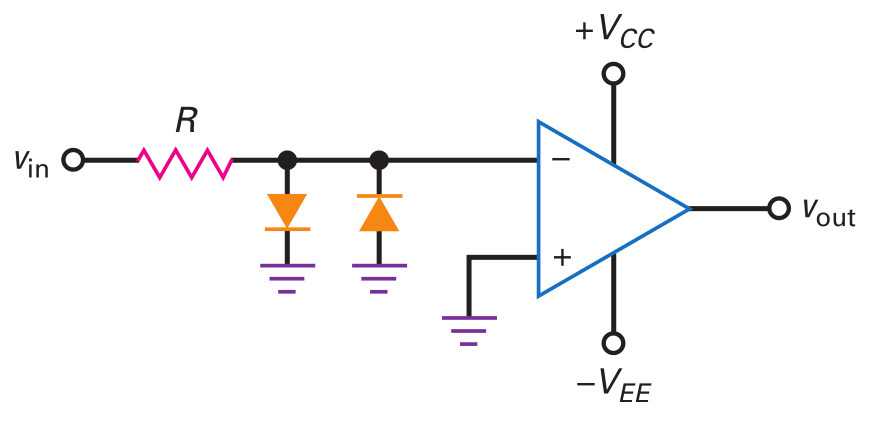
\includegraphics[width=\linewidth]{img/img04}
			\caption{Inverting comparator with clamping diodes}
			\label{fig:img04}
		\end{figure}
	\end{multicols}
\end{frame}
		
\begin{frame}{Inverting Comparator}
	\begin{multicols}{2}
		\begin{itemize}
			\item In this case, a slightly positive input voltage produces a maximum negative output, as shown in Fig. \ref{fig:img05}.
			\item On the other hand, a slightly negative input voltage produces a maximum positive output.
		\end{itemize}
		\begin{figure}
			\centering
			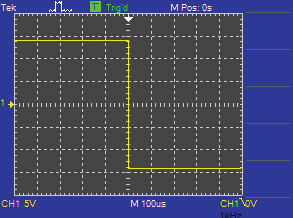
\includegraphics[width=\linewidth]{img/img05}
			\caption{Input/output response}
			\label{fig:img05}
		\end{figure}
	\end{multicols}
\end{frame}

\begin{frame}
	\frametitle{Diode Clamps}
	\begin{itemize}
		\item The use of diode clamps to protect sensitive circuits.
		\item Fig. \ref{fig:img04} is a practical example.
		\item We see two diode clamps protecting the comparator against excessively large input voltages.
		\item For instance, the LM311 is an IC comparator with an absolute maximum input rating of 615 V.
		\item If the input voltage exceeds these limits, the LM311 will be destroyed.
	\end{itemize}
\end{frame}

\begin{frame}{Diode Clamps}
	\begin{itemize}
		\item With some comparators, the maximum input voltage rating may be as little as $\pm$5 V, whereas with others it may be more than $\pm$30 V.
		\item In any case, we can protect a comparator against destructively large input voltages by using the diode clamps shown in Fig. \ref{fig:img04}. \item These diodes have no effect on the operation of the circuit as long as the magnitude of the input voltage is less than 0.7 V.
		\item When the magnitude of the input voltage is greater than 0.7 V, one of the diodes will turn on and clamp the magnitude of the inverting input voltage to approximately 0.7 V.
	\end{itemize}
\end{frame}

\begin{frame}{Diode Clamps}
	\begin{itemize}
		\item Some ICs are optimized for use as comparators.
		\item These IC comparators often have diode clamps built into their input stages.
		When using one of these comparators, we have to add an external resistor in series with the input terminal.
		\item This series resistor will limit the internal diode currents to a safe level.
	\end{itemize}
\end{frame}

\begin{frame}
	\frametitle{Converting Sine Waves to\\Square Waves}
	\begin{itemize}
		\item The \textbf{trip point} (also called the \textbf{threshold} or \textbf{reference}) of a comparator is the input voltage that causes the output voltage to switch states (from low to high or from high to low).
		\item In the noninverting and inverting comparators discussed earlier, the trip point is zero because this is the value of input voltage where the output switches states.
		\item Since a zero-crossing detector has a two-state output, any periodic input signal that crosses zero threshold will produce a rectangular output waveform.
	\end{itemize}
\end{frame}

\begin{frame}{Converting Sine Waves to\\Square Waves}
	\begin{multicols}{2}
		\begin{itemize}
			\item For instance, if a sine wave is the input to a noninverting comparator with a threshold of 0 V, the output will be the square wave shown in Fig. \ref{fig:img06}.
			\item As we can see, the output of a zero-crossing detector switches states each time the input voltage crosses the zero threshold.
		\end{itemize}
		\columnbreak
		\begin{figure}
			\centering
			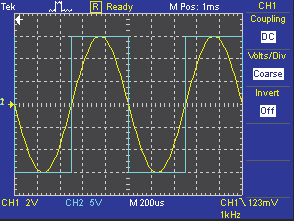
\includegraphics[width=\linewidth]{img/img06}
			\caption{Noninverting comparator converts sine waves to square waves}
			\label{fig:img06}
		\end{figure}
	\end{multicols}
\end{frame}

\begin{frame}{Converting Sine Waves to\\Square Waves}
	\begin{multicols}{2}
		\begin{itemize}
			\item Fig. \ref{fig:img07} shows the input sine wave and the output square wave for an inverting comparator with a threshold of 0 V.
			\item With this zero-crossing detector, the output square wave is 180$^{\circ}$ out of phase with the input sine wave.
		\end{itemize}
		\columnbreak
		\begin{figure}
			\centering
			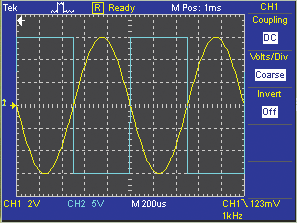
\includegraphics[width=\linewidth]{img/img07}
			\caption{Inverting comparator converts sine waves to square waves}
			\label{fig:img07}
		\end{figure}
	\end{multicols}
\end{frame}

\begin{frame}
	\frametitle{Linear Region}
	\begin{multicols}{2}
		\begin{itemize}
			\item Fig. \ref{fig:img08} shows a zero-crossing detector.
			\item If this comparator had an infinite open-loop gain, the transition between negative and positive saturation would be vertical.
			\item In Fig. \ref{fig:img03}, the transition appears to be vertical because the sensitivity of the 2 channel is 10 mV/Div.
		\end{itemize}
		\columnbreak
		\begin{figure}
			\centering
			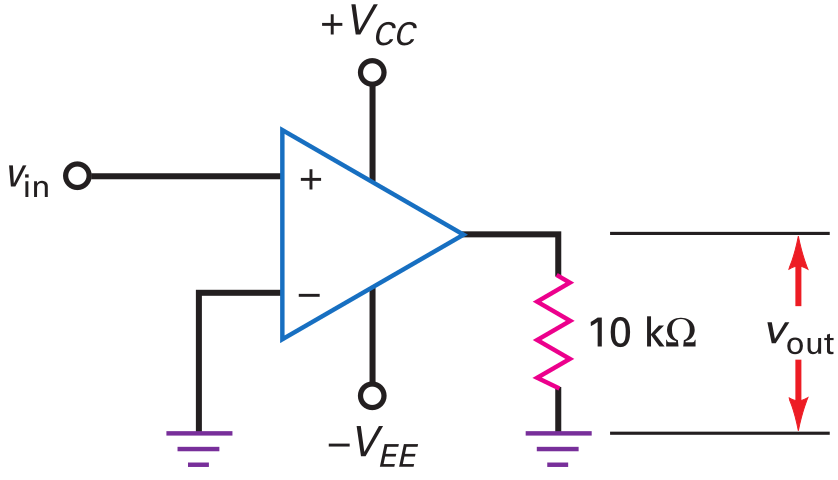
\includegraphics[width=\linewidth]{img/img08}
			\caption{Narrow linear region of typical comparator}
			\label{fig:img08}
		\end{figure}
	\end{multicols}
\end{frame}

\begin{frame}{Linear Region}
	\begin{itemize}
		\item When the sensitivity of the 2 channel is changed to 200 $\mu$V/Div, we can see that the transition is not vertical, as shown in Fig. \ref{fig:img09}.
	\end{itemize}
	\begin{figure}
		\centering
		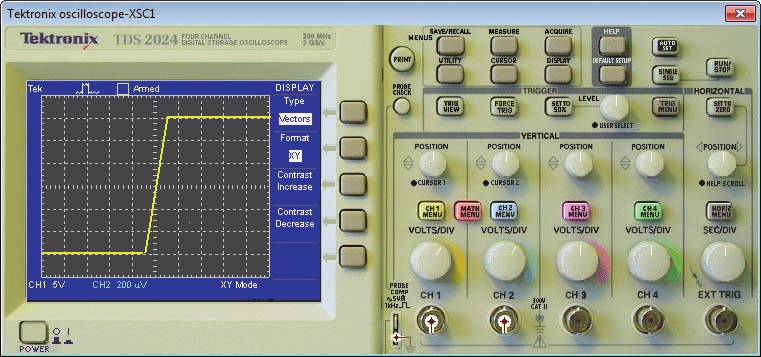
\includegraphics[width=0.8\linewidth]{img/img09}
		\caption{Narrow linear region of typical comparator}
		\label{fig:img09}
	\end{figure}
\end{frame}

\begin{frame}{Linear Region}
	\begin{itemize}
		\item It takes approximately $\pm$100 $\mu$V to get positive or negative saturation.
		\item This is typical for a comparator.
		\item The narrow input region between approximately -100 and +100 $\mu$V is called the \textbf{linear region of the comparator}.
		\item During a zero crossing, a changing input signal usually passes through the linear region so quickly that we see only a sudden jump between negative and positive saturation, or vice versa.
	\end{itemize}
\end{frame}

\begin{frame}
	\frametitle{Interfacing Analog and\\Digital Circuits}
	\begin{itemize}
		\item Comparators usually interface at their outputs with digital circuits such as CMOS, EMOS, or TTL (stands for transistor-transistor logic, a family of digital circuits).
	\end{itemize}
	\begin{multicols}{2}
		\begin{itemize}
			\item Fig. \ref{fig:205a} shows how a zero-crossing detector can interface with an EMOS circuit.
			\item Whenever the input voltage is greater than zero, the output of the comparator is high.
			This turns on the power FET and produces a large load current.
		\end{itemize}
		\begin{figure}
			\centering
			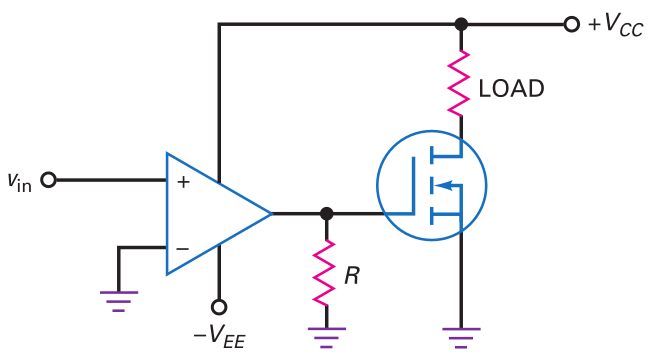
\includegraphics[width=\linewidth]{img/205a}
			\caption{Comparator interfaces with power FET}
			\label{fig:205a}
		\end{figure}
	\end{multicols}
\end{frame}

\begin{frame}{Interfacing Analog and\\Digital Circuits}
	\begin{multicols}{2}
		\begin{itemize}
			\item Fig. \ref{fig:205b} shows a zero-crossing detector interfacing with a CMOS inverter.
			\item The idea is basically the same.
			\item A comparator input greater than zero produces a high input to the CMOS inverter.
		\end{itemize}
		\begin{figure}
			\centering
			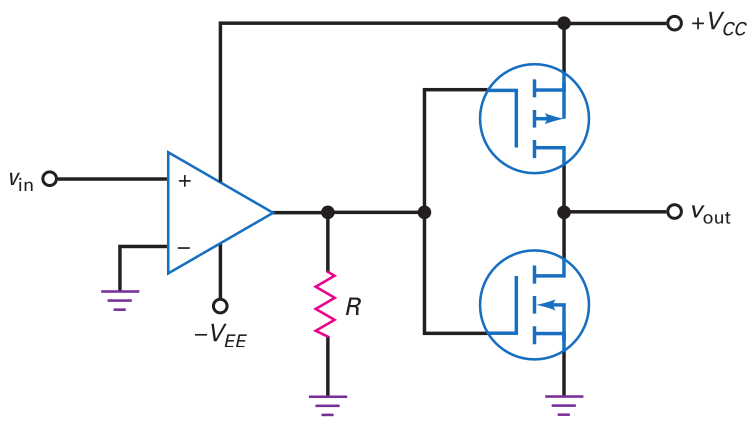
\includegraphics[width=\linewidth]{img/205b}
			\caption{Comparator interfaces with CMOS}
			\label{fig:205b}
		\end{figure}
	\end{multicols}
\end{frame}

\begin{frame}{Interfacing Analog and\\Digital Circuits}
	\begin{itemize}
		\item Most EMOS devices can handle input voltages greater than $\pm$15 V, and most CMOS devices can handle input voltages up to $\pm$15 V.
		\item Therefore, we can interface the output of a typical comparator without any level shifting or clamping.
		\item TTL logic, on the other hand, operates with lower input voltages.
		\item Because of this, interfacing a comparator with TTL requires a different approach (to be discussed in the next section).
	\end{itemize}
\end{frame}

\begin{frame}
	\frametitle{Clamping Diodes and Compensating Resistors}
	\begin{multicols}{2}
		\begin{itemize}
			\item When a current-limiting resistor is used with clamping diodes, a compensating resistor of equal size may be used on the other input of the comparator, as shown in Fig. \ref{fig:206}.
		\end{itemize}
		\columnbreak
		\begin{figure}
			\centering
			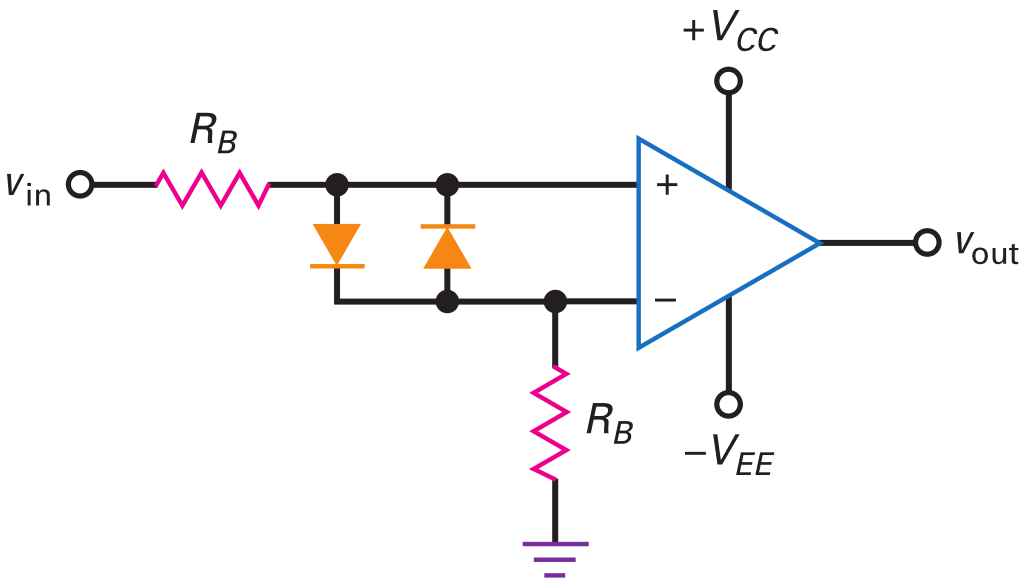
\includegraphics[width=\linewidth]{img/206}
			\caption{Using a compensating resistor to minimize the effect of $I_\text{in(bias)}$}
			\label{fig:206}
		\end{figure}
	\end{multicols}
\end{frame}

\begin{frame}{Clamping Diodes and Compensating Resistors}
	\begin{itemize}
		\item This is still a zero-crossing detector, except that it now has a compensating resistor to eliminate the effect of input bias current.
		\item As before, the diodes are normally off and have no effect on the operation of the circuit.
		It is only when the input tries to exceed $\pm$0.7 V that one of the clamping diodes turns on and protects the comparator against excessive input voltage.
	\end{itemize}
\end{frame}

\begin{frame}
	\frametitle{Bounded Output}
	\begin{itemize}
		\item The output swing of a zero-crossing detector may be too large in some applications.
		\item If so, we can bound the output by using back-to-back zener diodes, as shown in Fig. \ref{fig:207a}.
	\end{itemize}
	\begin{figure}
		\centering
		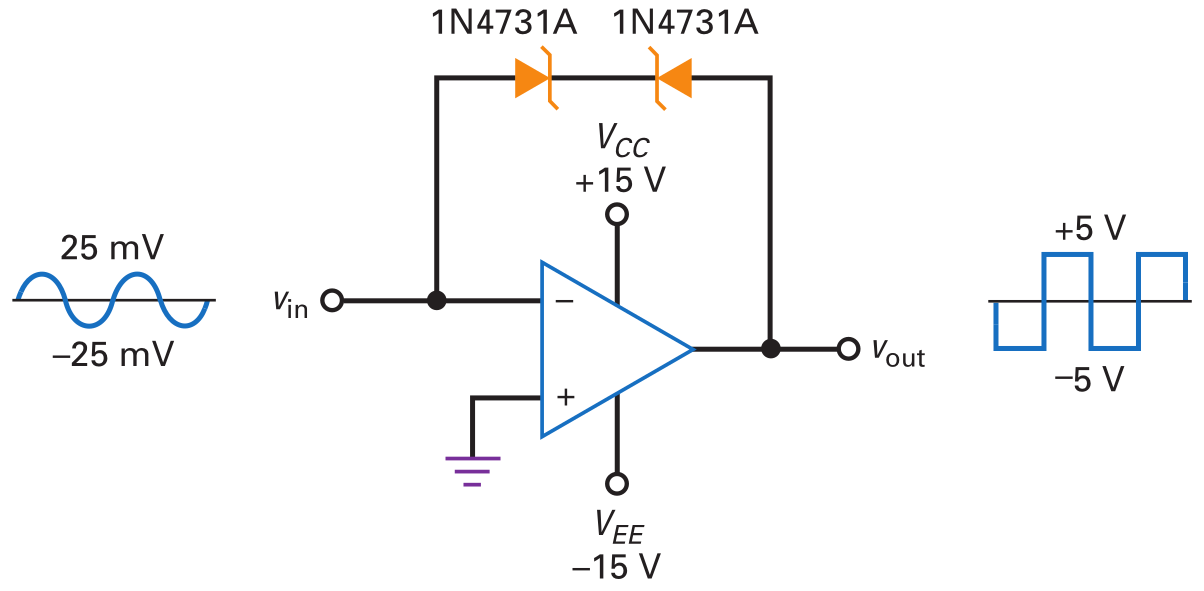
\includegraphics[width=0.7\linewidth]{img/207a}
		\caption{Bounded outputs using Zener diodes}
		\label{fig:207a}
	\end{figure}
\end{frame}

\begin{frame}{Bounded Output}
	\begin{itemize}
		\item In this circuit, as shown in Fig. \ref{fig:207a}, the inverting comparator has a bounded output because one of the diodes will be conducting in the forward direction and the other will be operating in the breakdown region.
		\item For instance, a 1N4731A has a zener voltage of 4.3 V.
		\item Therefore, the voltage across the two diodes will be approximately $\pm$5 V.
		\item If the input voltage is a sine wave with a peak value of 25 mV, then the output voltage will be an inverted square wave with a peak voltage of 5 V.
	\end{itemize}
\end{frame}

\begin{frame}{Bounded Output}
	\begin{itemize}
		\item Fig. \ref{fig:207b} shows another example of a bounded output.
		\item This time, the output diode will clip off the negative half-cycles of the output voltage.
		\item Given an input sine wave with a peak of 25 mV, the output is bounded between -0.7 and +15 V as shown.
	\end{itemize}
	\begin{figure}
		\centering
		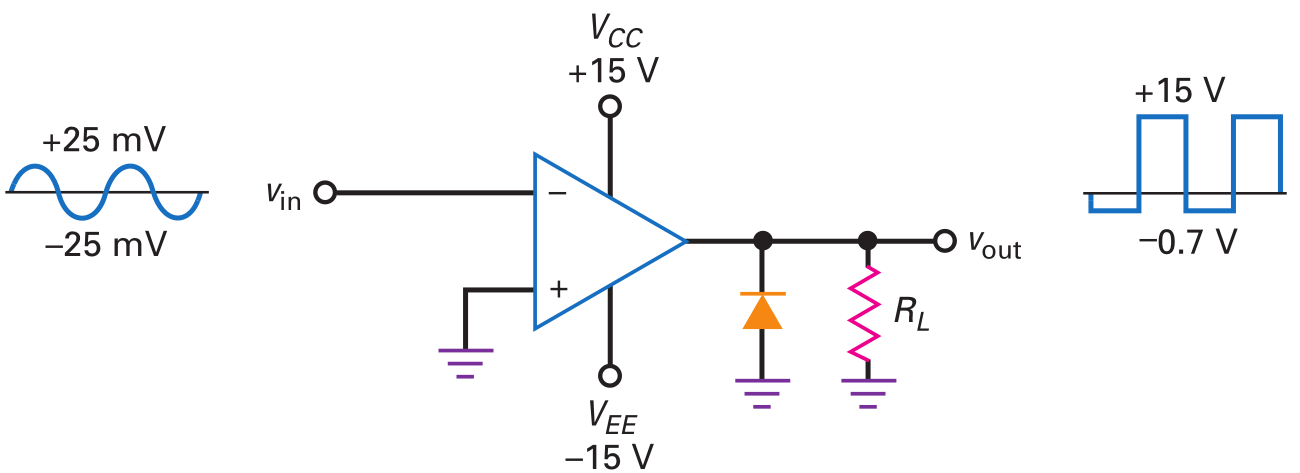
\includegraphics[width=0.8\linewidth]{img/207b}
		\caption{Bounded outputs using rectifier diode}
		\label{fig:207b}
	\end{figure}
\end{frame}

\begin{frame}
	\frametitle{Bounded Output}
	\centering
	~ TIME TO QUIZIZZ ~
\end{frame}

\section{Comparators with Nonzero Reference}

\begin{frame}
	\frametitle{Introduction}
	\begin{itemize}
		\item In some applications, a threshold voltage different from zero may be preferred.
		\item By biasing either input, we can change the threshold voltage as needed.
	\end{itemize}
\end{frame}

\begin{frame}
	\frametitle{Moving the Trip Point}
	\begin{multicols}{2}
		\begin{itemize}
			\item In Fig. \ref{fig:2011a}, a voltage divider produces the following reference voltage for the
			inverting input:
			\begin{equation}\label{eq:202}
				v_{ref} = \frac{R_2}{R_1 + R_2} V_{CC}
			\end{equation}
		\end{itemize}
		\columnbreak
		\begin{figure}
			\centering
			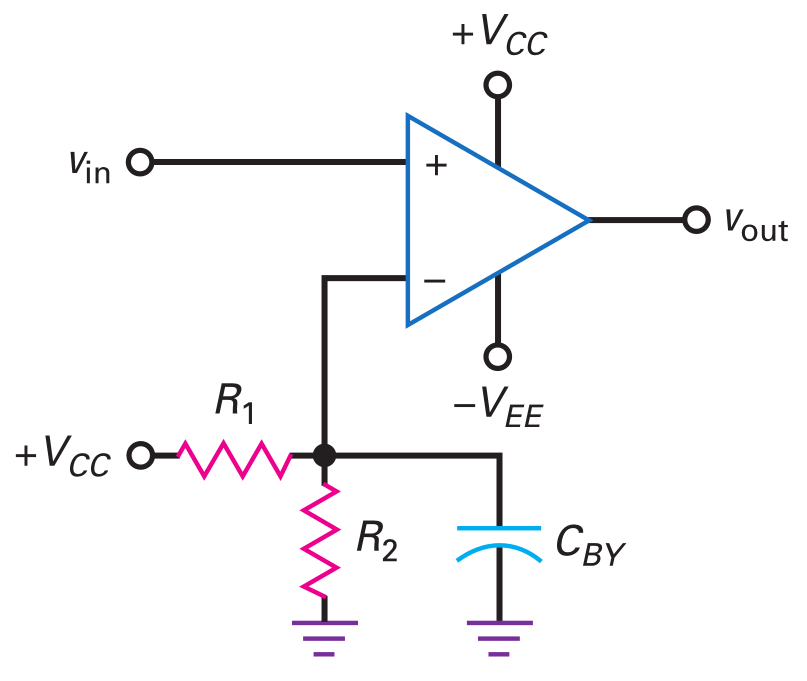
\includegraphics[width=\linewidth]{img/2011a}
			\caption{Positive threshold}
			\label{fig:2011a}
		\end{figure}
	\end{multicols}
\end{frame}

\begin{frame}{Moving the Trip Point}
	\begin{itemize}
		\item When $v_{in}$ is greater than $v_{ref}$, the differential input voltage is positive and the output voltage is high. When $v_{in}$ is less than $v_{ref}$, the differential input voltage is negative and the output voltage is low.
		\item A bypass capacitor is typically used on the inverting input, as shown in Fig. \ref{fig:2011a}. 
		\item This reduces the amount of power-supply ripple and other noise appearing at the inverting input.
	\end{itemize}
\end{frame}

\begin{frame}{Moving the Trip Point}
	\begin{itemize}
		\item To be effective, the cutoff frequency of this bypass circuit should be much lower than the ripple frequency of the power supply.
		\item The cutoff frequency is given by:
		\begin{equation}\label{eq:203}
			f_c = \frac{1}{2 \pi (R_1 || R_2) C_{BY}}
		\end{equation}
	\end{itemize}
\end{frame}

\begin{frame}{Moving the Trip Point}
	\begin{multicols}{2}
		\begin{itemize}
			\item Figure \ref{fig:2011b} shows the transfer characteristic (input/output response).
			\item The trip point is now equal to $v_{ref}$.
			\item When $v_{in}$ is greater than $v_{ref}$, the output of the comparator goes into positive saturation.
			\item When $v_{in}$ is less than $v_{ref}$, the output goes into negative saturation.
		\end{itemize}
		\columnbreak
		\begin{figure}
			\centering
			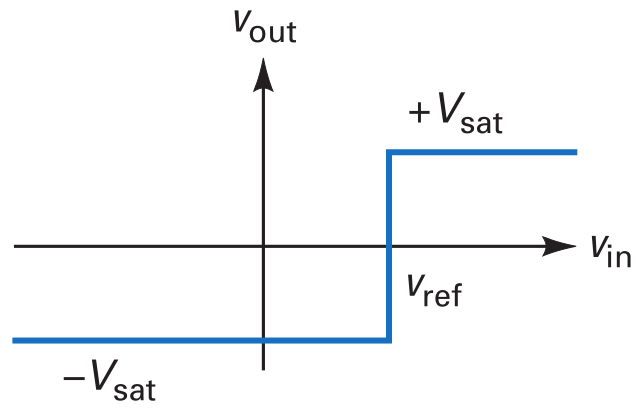
\includegraphics[width=\linewidth]{img/2011b}
			\caption{Positive input/output response}
			\label{fig:2011b}
		\end{figure}
	\end{multicols}
\end{frame}

\begin{frame}{Moving the Trip Point}
		\begin{itemize}
			\item A comparator like this is sometimes called a limit detector because a positive output indicates that the input voltage exceeds a specific limit.
			\item With different values of $R_1$ and $R_2$, we can set the limit anywhere between 0 and $V_{CC}$.
		\end{itemize}
\end{frame}

\begin{frame}{Moving the Trip Point}
	\begin{multicols}{2}
		\begin{itemize}
			\item If a negative limit is preferred, connect $-V_{EE}$ to the voltage divider, as shown in Fig. \ref{fig:2011c}.
			\item Now a negative reference voltage is applied to the inverting input.
		\end{itemize}
		\vfill\null
		\columnbreak
		\begin{figure}
			\centering
			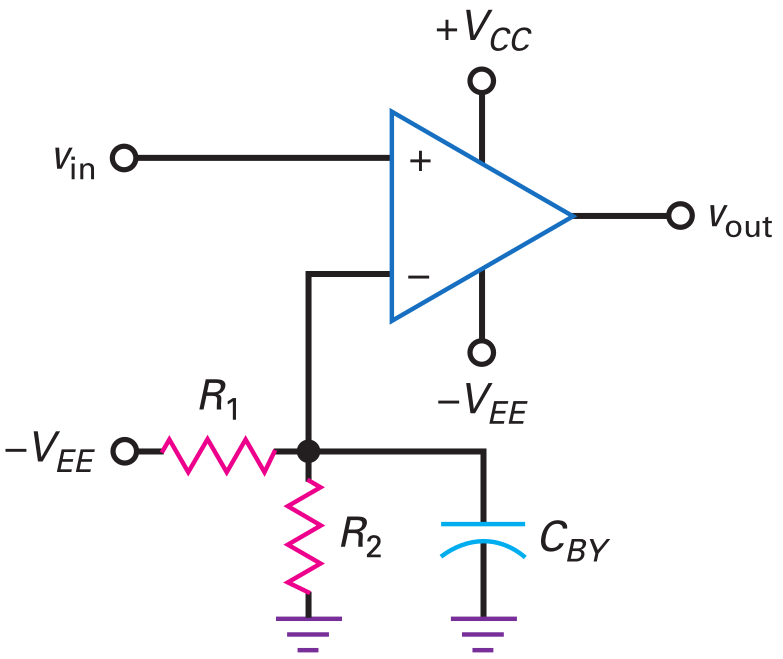
\includegraphics[width=\linewidth]{img/2011c}
			\caption{Negative threshold}
			\label{fig:2011c}
		\end{figure}
	\end{multicols}
\end{frame}

\begin{frame}{Moving the Trip Point}
	\begin{multicols}{2}
		\begin{itemize}
			\item When $v_{in}$ is more positive than $v_{ref}$, the differential input voltage is positive and the output is high, as shown in Fig. \ref{fig:2011d}.
			\item When $v_{in}$ is more negative than $v_{ref}$, the output is low.
		\end{itemize}
		\vfill\null
		\columnbreak
		\begin{figure}
			\centering
			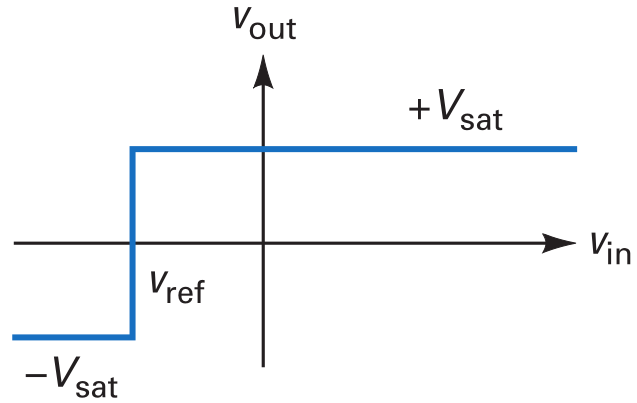
\includegraphics[width=\linewidth]{img/2011d}
			\caption{Negative input/output}
			\label{fig:2011d}
		\end{figure}
	\end{multicols}
\end{frame}

\begin{frame}
	\frametitle{Single-Supply Comparator}
	\begin{multicols}{2}
		\begin{itemize}
			\item A typical op amp like the 741C can run on a single positive supply by grounding the
			$-V_{EE}$ pin, as shown in Fig. \ref{fig:2012a}.
			\item The output voltage has only one polarity, either a low or a high positive voltage.
			\item For instance, with $V_{CC}$ equal to +15 V, the output swing is from approximately +1.5 V (low state) to around +13.5 V (high state).
		\end{itemize}
		\vfill\null
		\columnbreak
		\begin{figure}
			\centering
			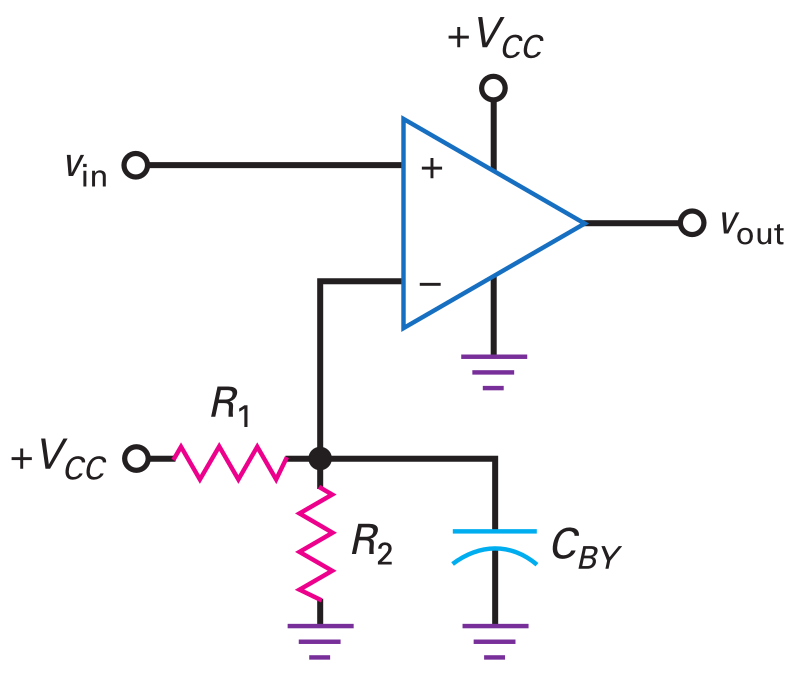
\includegraphics[width=\linewidth]{img/2012a}
			\caption{Single-supply comparator}
			\label{fig:2012a}
		\end{figure}
	\end{multicols}
\end{frame}

\begin{frame}{Single-Supply Comparator}
	\begin{multicols}{2}
		\begin{itemize}
			\item When $v_{in}$ is greater than $v_{ref}$, the output is high, as shown in Fig. \ref{fig:2012b}.
			\item When $v_{in}$ is less than $v_{ref}$, the output is low. In either case, the output has a positive polarity.
			\item For many digital applications, this kind of positive output is preferred
		\end{itemize}
		\vfill\null
		\columnbreak
		\begin{figure}
			\centering
			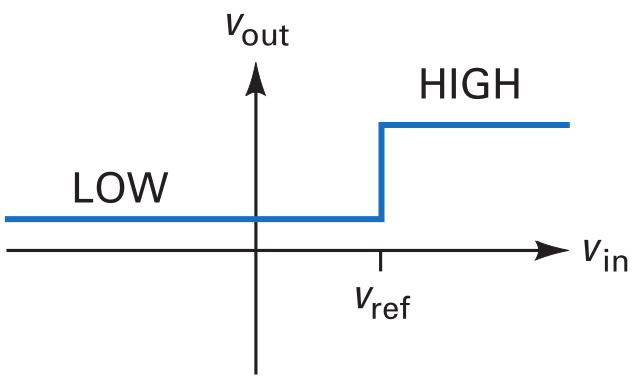
\includegraphics[width=\linewidth]{img/2012b}
			\caption{Input/output responser}
			\label{fig:2012b}
		\end{figure}
	\end{multicols}
\end{frame}

\begin{frame}
	\frametitle{IC Comparators}
	\begin{itemize}
		\item An op amp like a 741C can be used as a comparator, but it has speed limitations
		because of its slew rate.
		\item With a 741C, the output can change no faster than 0.5 V/$\mu$s.
		\item Because of this, a 741C takes more than 50 $\mu$s to switch output states with
		supplies of $\pm$15 V.
		\item One solution to the slew-rate problem is to use a faster op amp like an LM318.
		Since it has a slew rate of 70 V/$\mu$s, it can switch from $-V_{sat}$ to $+V_{sat}$ in approximately 0.3 $\mu$s.
	\end{itemize}
\end{frame}

\begin{frame}{IC Comparators}
	\begin{itemize}
			\item Another solution is to eliminate the compensating capacitor found in a typical op amp.
			\item Since a comparator is always used as a nonlinear circuit, a compensating capacitor is unnecessary.
			\item A manufacturer can delete the compensating capacitor and significantly increase the slew rate.
			\item When an IC has been optimized for use as a comparator, the device is listed in a separate section of the manufacturer's data book.
			\item This is why you will find a section on op amps and another section on comparators in the typical data book.
	\end{itemize}
\end{frame}

\begin{frame}
	\frametitle{Open-Collector Devices}
	\begin{multicols}{2}
		\begin{itemize}
			\item Fig. \ref{fig:2013a} is a simplified schematic diagram for an \textbf{open-collector comparator}.
			\item Notice that it runs off a single positive supply.
			\item The input stage is a diff amp ($Q_1$ and $Q_2$).
			\item A current source $Q_6$ supplies the tail current.
		\end{itemize}
		\vfill\null
		\begin{figure}
			\centering
			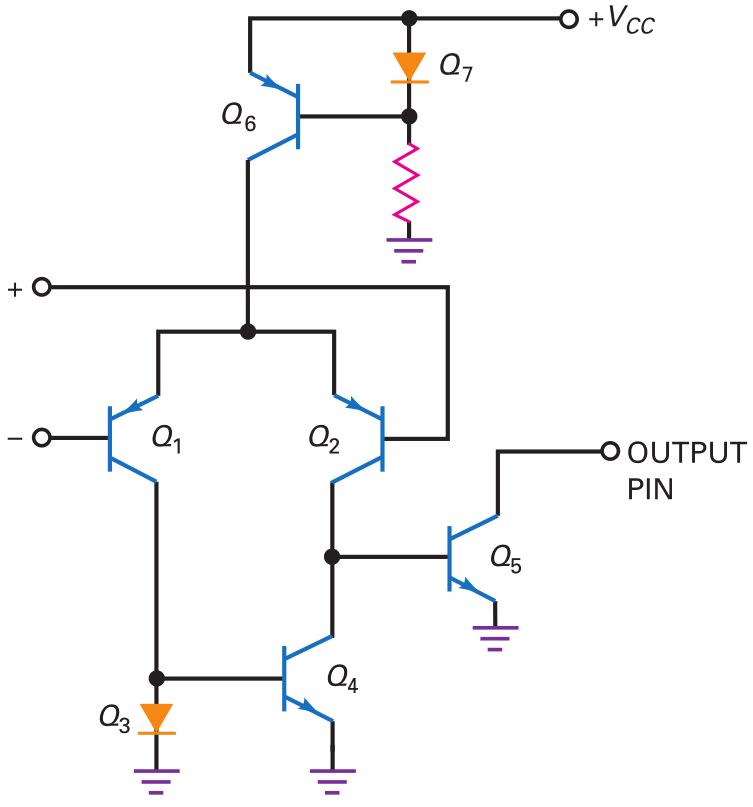
\includegraphics[width=\linewidth]{img/2013a}
			\caption{Simplified schematic diagram of IC comparator}
			\label{fig:2013a}
		\end{figure}
	\end{multicols}
\end{frame}

\begin{frame}{Open-Collector Devices}
	\begin{itemize}
		\item The diff amp drives an active-load $Q_4$.
		\item The output stage is a single transistor $Q_5$ with an open collector.
		\item This open collector allows the user to control the output swing of the comparator.
	\end{itemize}
\end{frame}

\begin{frame}{Open-Collector Devices}
	\begin{itemize}
		\item A typical op amp has an output stage that can be described as an active-pullup stage because it contains two devices in a Class-B push-pull connection.
		\item With the active pullup, the upper device turns on and pulls the output up to the high output state.
		\item On the other hand, an open-collector output stage of Fig. \ref{fig:2013a} needs external components to be connected to it.
	\end{itemize}
\end{frame}

\begin{frame}{Open-Collector Devices}
	\begin{multicols}{2}
		\begin{itemize}
			\item For the output stage to work properly, the user has to connect the open collector to an external resistor and supply voltage, as shown in Fig. \ref{fig:2013b}.
		\end{itemize}
		\vfill \null
		\columnbreak
		\begin{figure}
			\centering
			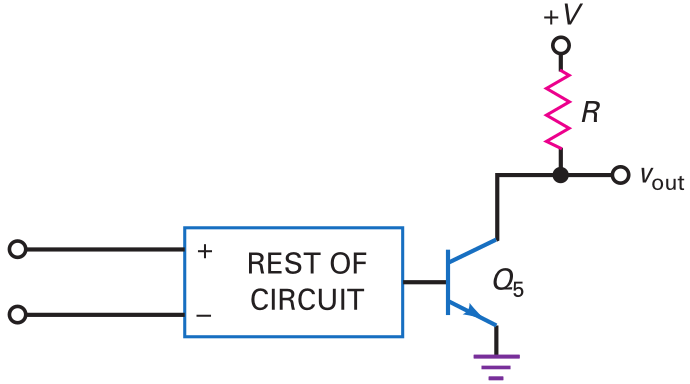
\includegraphics[width=\linewidth]{img/2013b}
			\caption{using pullup resistor with open-collector output stage}
			\label{fig:2013b}
		\end{figure}
	\end{multicols}
\end{frame}

\begin{frame}{Open-Collector Devices}
	\begin{itemize}
		\item The resistor is called a pullup resistor (Fig. \ref{fig:2013b}) because it pulls the output voltage up to the
		supply voltage when $Q_5$ is cut off.
		\item When $Q_5$ is saturated, the output voltage is low.
		\item Since the output stage is a transistor switch, the comparator produces a two-state output.
	\end{itemize}
\end{frame}

\begin{frame}{Open-Collector Devices}
	\begin{itemize}
		\item With no compensating capacitor in the circuit, the output in Fig. \ref{fig:2013a} can slew very rapidly because only small stray capacitances remain in the circuit.
		\item The main limitation on the switching speed is the amount of capacitance across $Q_5$.
		\item This output capacitance is the sum of the internal collector capacitance and the external stray wiring capacitance.
	\end{itemize}
\end{frame}

\begin{frame}{Open-Collector Devices}
	\begin{itemize}
		\item The output time constant is the product of the pullup resistance and the output capacitance. 
		\item For this reason, the smaller the pullup resistance in Fig. \ref{fig:2013b}, the faster the output voltage can change.
		Typically, $R$ is from a couple of hundred to a couple of thousand ohms.
	\end{itemize}
\end{frame}			

\begin{frame}{Open-Collector Devices}
	\begin{itemize}
		\item Examples of IC comparators are the LM311, LM339, and NE529.
		\item They all have an open-collector output stage, which means that you have to connect the output pin to a pullup resistor and a positive supply voltage.
		\item Because of their high slew rates, these IC comparators can switch output states in a microsecond or less.
	\end{itemize}
\end{frame}

\begin{frame}{Open-Collector Devices}
	\begin{itemize}
		\item The LM339 is a \textit{quad comparator}—four comparators in a single IC package. 
		\item It can run off a single supply or off dual supplies.
		\item Because it is inexpensive and easy to use, the LM339 is a popular comparator for general-purpose applications.
	\end{itemize}
\end{frame}

\begin{frame}{Open-Collector Devices}
	\begin{itemize}
		\item Not all IC comparators have an open-collector output stage.
		\item Some, like the LM360, LM361, and LM760, have an active-collector output stage.
		\item The active pullup produces faster switching.
		\item These high-speed IC comparators require dual supplies.
	\end{itemize}
\end{frame}

\begin{frame}
	\frametitle{Driving TTL}
	\begin{multicols}{2}
		\begin{itemize}
			\item The LM339 is an open-collector device.
			\item Fig. \ref{fig:2014a} shows how an LM339 can be connected to interface with TTL devices.
			\item A positive supply of +15 V is used for the comparator, but the open collector of the LM339 is connected to a supply of +5 V through a pullup resistor of 1 k$\Omega$.
		\end{itemize}
		\vfill\null
		\begin{figure}
			\centering
			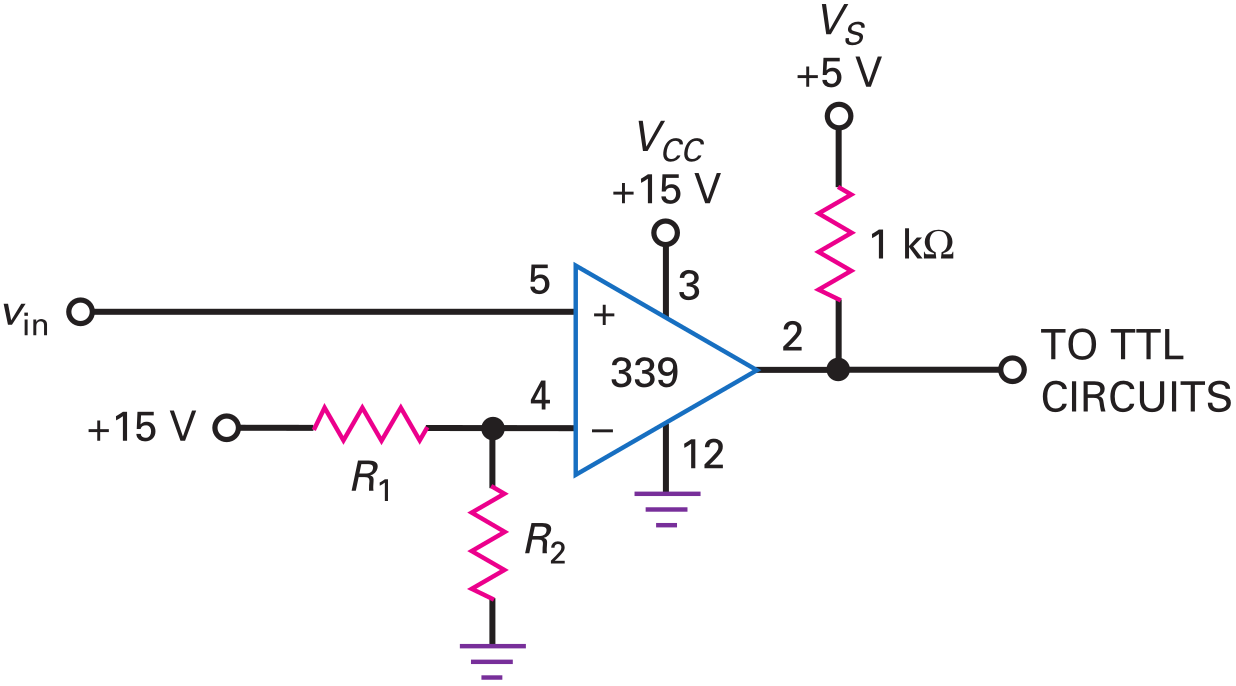
\includegraphics[width=\linewidth]{img/2014a}
			\caption{LM339 comparator}
			\label{fig:2014a}
		\end{figure}
	\end{multicols}
\end{frame}

\begin{frame}{Driving TTL}
	\begin{multicols}{2}
		\begin{itemize}
			\item Because of this, the output swings between 0 and +5 V, as shown in Fig. \ref{fig:2014b}.
			\item This output signal is ideal for TTL devices because they are designed to work with supplies of +5 V.
		\end{itemize}
		\vfill\null
		\begin{figure}
			\centering
			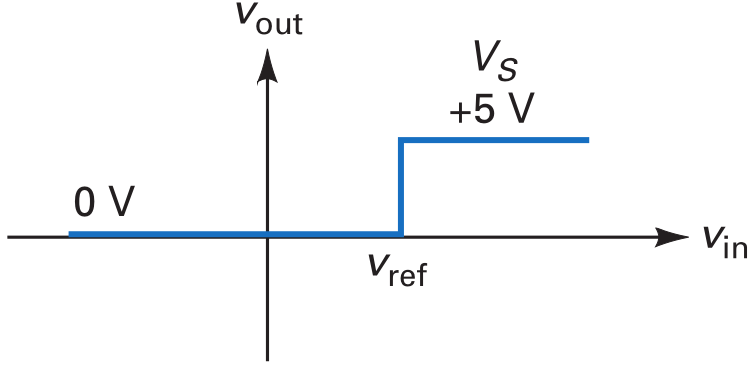
\includegraphics[width=\linewidth]{img/2014b}
			\caption{input/output response}
			\label{fig:2014b}
		\end{figure}
	\end{multicols}
\end{frame}

\section{Comparators with Hysteresis}

\begin{frame}
	\frametitle{Introduction}
	\begin{itemize}
		\item If the input to a comparator contains a large amount of noise, the output will be erratic when vin is near the trip point.
		\item One way to reduce the effect of noise is by using a comparator with positive feedback. The positive feedback produces two separate trip points that prevent a noisy input from producing false transitions.
	\end{itemize}
\end{frame}

\begin{frame}
	\frametitle{Noise}
	\begin{itemize}
		\item \textit{Noise} is any kind of unwanted signal that is not derived from or harmonically related to the input signal.
		\item Electric motors, neon signs, power lines, car ignitions, lightning, and so on produce electromagnetic fields that can induce noise voltages into electronic circuits.
		\item Power-supply ripple is also classified as noise since it is not related to the input signal. 
		\item By using regulated power supplies and shielding, we usually can reduce the ripple and induced noise to an acceptable level.
	\end{itemize}
\end{frame}

\begin{frame}{Noise}
	\begin{multicols}{2}
		\begin{itemize}
			\item Thermal noise, on the other hand, is caused by the random motion of free electrons inside a resistor (see Fig. \ref{fig:2016a}).
			\item The energy for this electron motion comes from the thermal energy of the surrounding air.
			\item The higher the ambient temperature, the more active the electrons.
		\end{itemize}
		\vfill\null
		\columnbreak
		\begin{figure}
			\centering
			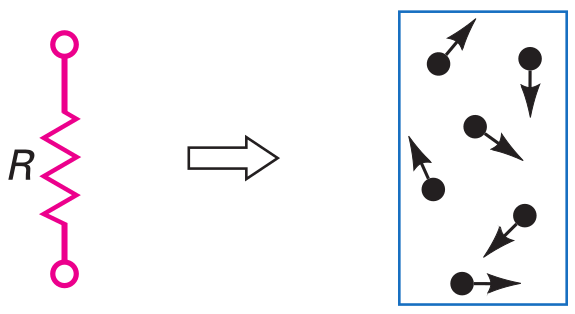
\includegraphics[width=\linewidth]{img/2016a}
			\caption{Thermal noise: Random electron motion in resistor}
			\label{fig:2016a}
		\end{figure}
	\end{multicols}
\end{frame}

\begin{frame}{Noise}
	\begin{multicols}{2}
		\begin{itemize}
			\item The motion of billions of free electrons inside a resistor is pure chaos.
			\item At some instants, more electrons move up than down, producing a small negative voltage across the resistor.
			\item At other instants, more electrons move down than up, producing a positive voltage.
			\item If this type of noise were amplified and viewed on an oscilloscope, it would resemble Fig. \ref{fig:2016b}.
			\item Like any voltage, noise has an rms or effective value.
			\item As an approximation, the highest noise peaks are about four times the rms value.
		\end{itemize}
		\begin{figure}
			\centering
			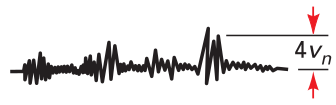
\includegraphics[width=\linewidth]{img/2016b}
			\caption{Thermal noise: noise on oscilloscope.}
			\label{fig:2016b}
		\end{figure}
	\end{multicols}
\end{frame}

\begin{frame}{Noise}
	\begin{itemize}
		\item The randomness of the electron motion inside a resistor produces a distribution of noise at virtually all frequencies.
		\item The rms value of this noise increases with temperature, bandwidth, and resistance.
		\item For our purposes, we need to be aware of how noise may affect the output of a comparator.
	\end{itemize}
\end{frame}

\begin{frame}
	\frametitle{Noise Triggering}
	\begin{itemize}
		\item As discussed in Sec. 20-1, the high open-loop gain of a comparator means that an input of only 100 $\mu$V may be enough to switch the output from one state to another.
		\item If the input contains noise with a peak of 100 $\mu$V or more, the comparator will detect the zero crossings produced by the noise.
	\end{itemize}
\end{frame}

\begin{frame}{Noise Triggering}
	\begin{multicols}{2}
		\begin{itemize}
			\item Fig. \ref{fig:2017} shows the output of a comparator with no input signal, except for noise.
			\item When the noise peaks are large enough, they produce unwanted changes in the comparator output.
			\item For instance, the noise peaks at A, B, and C are producing unwanted transitions from low to high.
			\item When an input signal is present, the noise is superimposed on the input signal and produces erratic triggering.
		\end{itemize}
		\begin{figure}
			\centering
			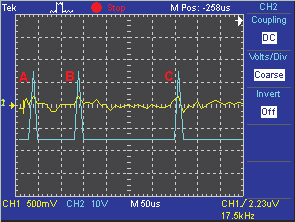
\includegraphics[width=\linewidth]{img/2017}
			\caption{Noise produces false triggering of comparator.}
			\label{fig:2017}
		\end{figure}
	\end{multicols}
\end{frame}

\begin{frame}
	\frametitle{Schmitt Trigger}
	\begin{itemize}
		\item The standard solution for a noisy input is to use a comparator like the one shown in Fig. \ref{fig:2018}(a).
		\item The input voltage is applied to the inverting input.
		\item Because the feedback voltage at the noninverting input is aiding the input voltage, the feed-back is positive.
		\item A comparator using positive feedback like this is usually called a Schmitt trigger.
	\end{itemize}
\end{frame}

\begin{frame}{Schmitt Trigger}
	\begin{figure}
		\centering
		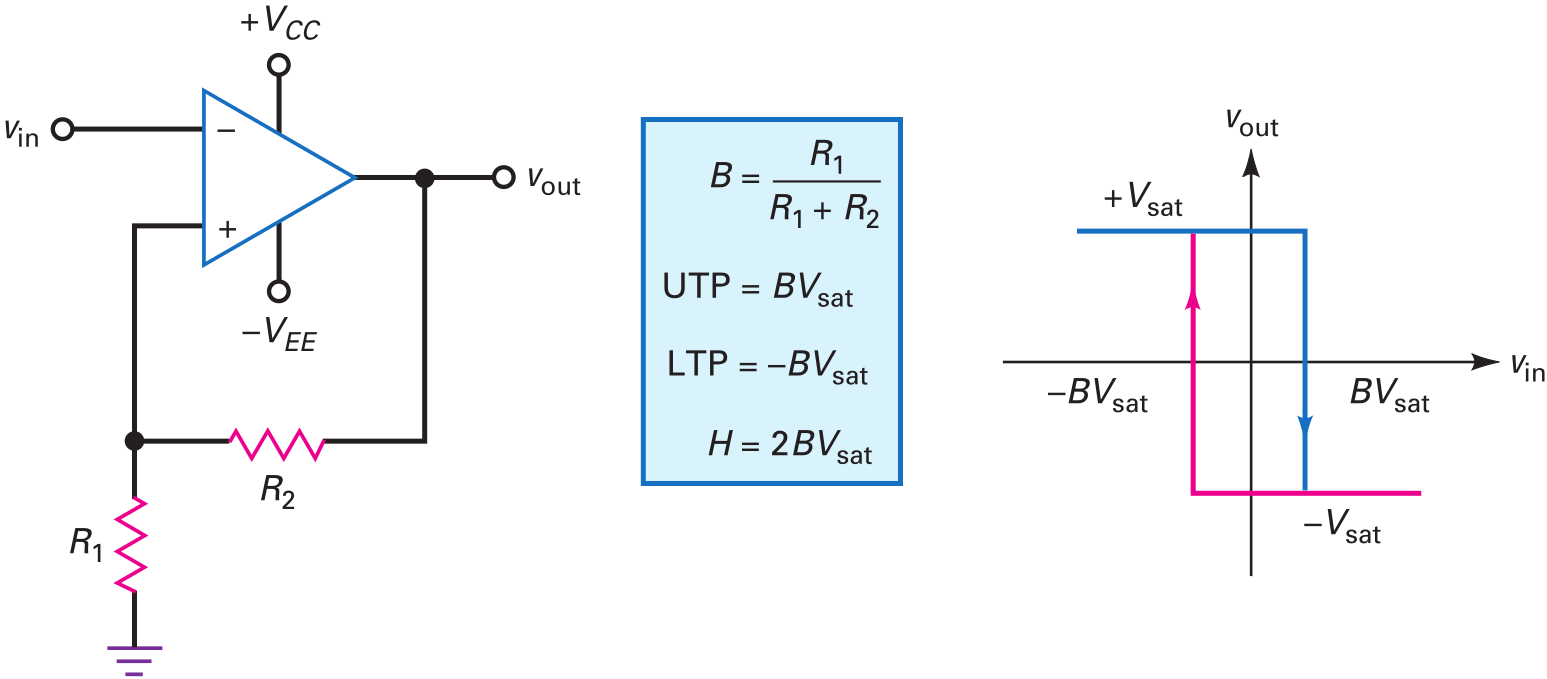
\includegraphics[width=\linewidth]{img/2018}
		\caption{(a) Inverting Schmitt trigger; (b) input/output response has hysteresis.}
		\label{fig:2018}
	\end{figure}
\end{frame}

\begin{frame}{Schmitt Trigger}
	\begin{itemize}
		\item When the comparator is positively saturated, a positive voltage is fed back to the noninverting input.
		\item This positive feedback voltage holds the output in the high state.
		\item Similarly, when the output voltage is negatively saturated, a negative voltage is fed back to the noninverting input, holding the output in the low state.
		\item In either case, the positive feedback reinforces the existing output state.
	\end{itemize}
\end{frame}

\begin{frame}{Schmitt Trigger}
	\begin{itemize}
		\item The feedback fraction is:
		\begin{equation}\label{eq:204}
			B = \frac{R_1}{R_1 + R_2}
		\end{equation}
		\item When the output is positively saturated, the reference voltage applied to the non-		inverting input is:
		\begin{equation}\label{eq:205}
			v_{ref} = +BV_{sat}
		\end{equation}
		\item When the output is negatively saturated, the reference voltage is:
		\begin{equation}\label{eq:205}
			v_{ref} = -BV_{sat}
		\end{equation}
	\end{itemize}
\end{frame}

\begin{frame}{Schmitt Trigger}
	\begin{itemize}
		\item The output voltage will remain in a given state until the input voltage exceeds the reference voltage for that state.
		\item For instance, if the output is positively saturated, the reference voltage is $+BV_{sat}$.
		\item The input voltage must be increased to slightly more than $+BV_{sat}$ to switch the output voltage from positive to negative, as shown in Fig. \ref{fig:2018}(b).
		\item Once the output is in the negative state, it will remain there indefinitely until the input voltage becomes more negative than $-BV_{sat}$.
		\item Then, the output switches from negative to positive (Fig. \ref{fig:2018}(b)).
	\end{itemize}
\end{frame}

\begin{frame}
	\frametitle{Hysteresis}
	\begin{itemize}
		\item The unusual response of Fig. \ref{fig:2018}(b) has a useful property called hysteresis.
		\item To understand this concept, put your finger on the upper end of the graph where it says $+V_{sat}$.
		\item Assume that this is the current value of output voltage.
		\item Move your finger to the right along the horizontal line.
		\item Along this horizontal line, the input voltage is changing but the output voltage is still equal to $+V_{sat}$.
		\item When you reach the upper-right corner, $v_{in}$ equals $+BV_{sat}$.
		\item When $v_{in}$ increases to slightly more than $+BV_{sat}$, the output voltage goes into the transition region between the high and the low states.
	\end{itemize}
\end{frame}

\end{document}
